%!TEX TS-program = xelatex
\documentclass[a4paper, 12pt]{article}
\usepackage{barinovxesimple}
\geometry{top=25mm}
\geometry{bottom=35mm}
\geometry{left=35mm}
\geometry{right=20mm}
\setlist{labelindent=\parindent,leftmargin=*}
\begin{document}
\thispagestyle{empty}
\begin{center}
    \textit{Федеральное государственное автономное образовательное\\ учреждение высшего образования }

    \vspace{0.5ex}

        \textbf{«Московский физико-технический институт\\ (национальный исследовательский университет)»}
\end{center}

\vspace{10ex}

\begin{center}
    \vspace{13ex}

    \so{\textbf{Лабораторная работа №_._._}}

    \vspace{1ex}

    по курсу общей физики

    на тему:

    \textbf{\textit{<<>>}}

    \vspace{30ex}

    \begin{flushright}
        \noindent
        \textit{Работу выполнил:}\\  
        \textit{Баринов Леонид \\(группа Б02-827)}
    \end{flushright}
    \vfill
    Долгопрудный \\2019
\newpage
\setcounter{page}{1}
\fancyhead[R]{\nouppercase{\leftmark}}	
\end{center}

\section{Аннотация}
В работе будет проведено исследование энергетического спектра
$\gamma$-квантов, рассеянных на графите. Определена зависимость
энергии рассеянных $\gamma$-квантов в от угла рассеяния, а также будет
получена энергия покоя частиц, на которых происходит комптоновское
рассеяние.






\section{Теоретические сведения}
\emph{Эффект Комптона} --- увеличение длины волны рассеянного
излучения по сравнению с падающим. Интерпретируется как результат
упругого соударения двух частиц: $\gamma$-кванта (фотона) и свободного
электрона.

\begin{wrapfigure}{l}{0.3\linewidth}
    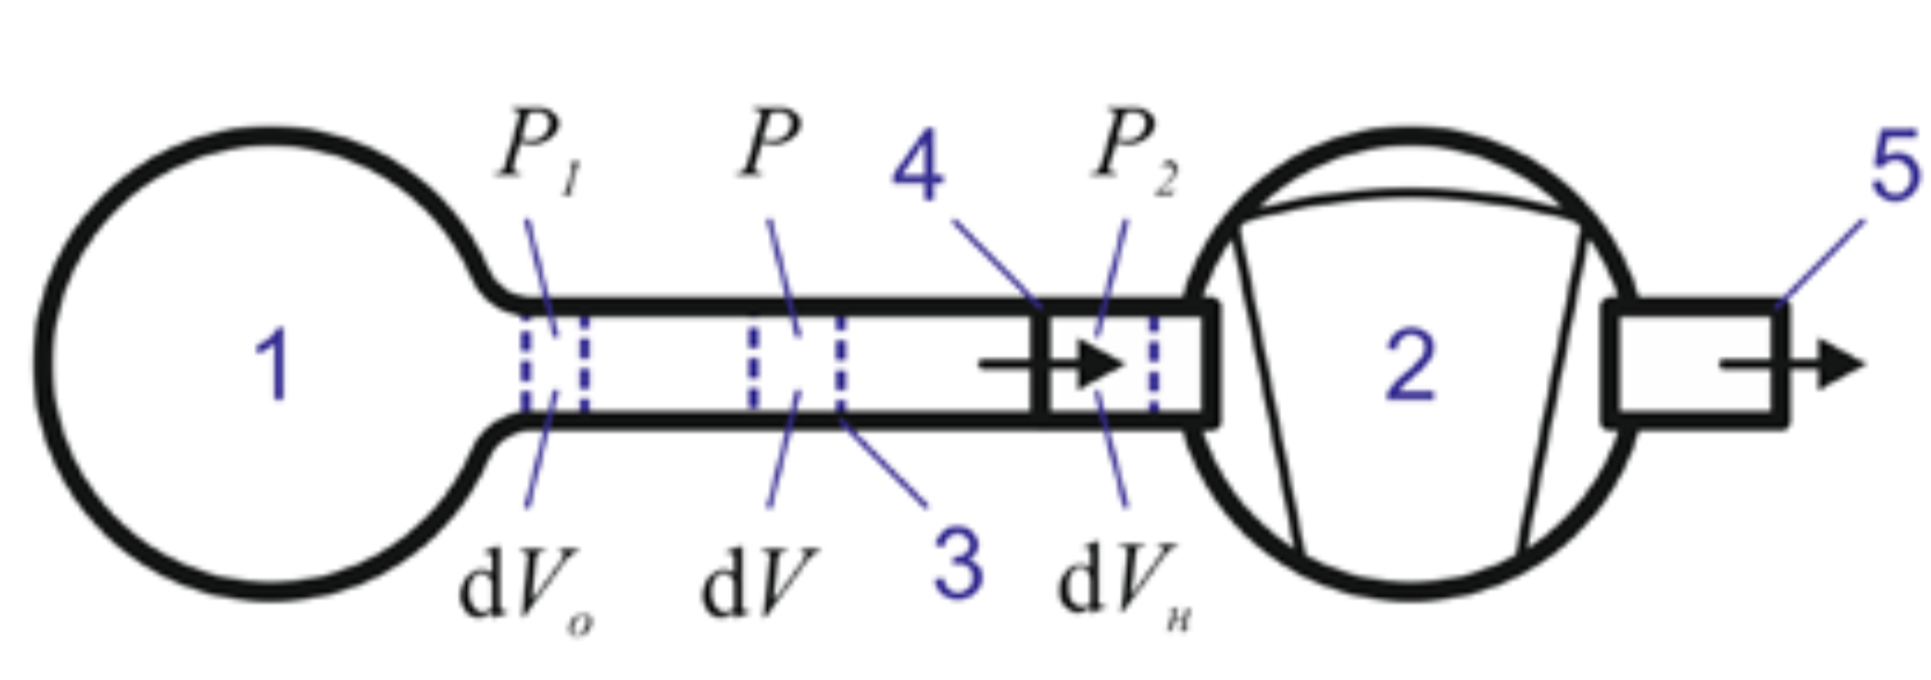
\includegraphics[width=\linewidth]{1}
    \caption{Векторная диаграмма рассеяния $\gamma$-кванта на
    электроне}
    \label{fig:1}
\end{wrapfigure}


Пусть электрон до соударения покоился, а $\gamma$-квант имел начальную
энергию $\hbar \omega_0$ и импульс $\hbar \omega_0 /c$. После
соударения электрон приобретает энергию $\gamma m c^2$ и импульс
$\gamma m v$, где $\gamma = 1/\sqrt{1-\beta^2}$, $\beta = v/c$, а
$\gamma$-квант рассеивается на некоторый угол $\theta$ по отношению к
первоначальному направлению движения. Энергия и импульс
$\gamma$-кванта становят соответственно равными $\hbar \omega_1$ и
$\hbar \omega_1 /c$ \ffig{fig:1}. 







\section{Оборудование}







\section{Результаты измерений и обработка результатов}







\section{Обсуждение результатов и выводы}













\end{document}
